\chapter{随机区域池化}
\label{cha:sap}

\section{引言}
\label{sec:sap:introduction}

对于绝大部分机器学习算法,特征表达能力~\cite{bengio2013representation}具有至关重要的作用,特征直接反映着对输入数据统计分布和个体差异的理解。以视觉物体识别任务为例,有效的特征表达形式,可以极大地简化网络后端的分类算法,提高网络的识别率。长期以来,图像的特征提取往往是人工设计的,虽然已经提出了一些具有不变性(如大小,尺度,旋转,光照等)的特征,例如SIFT~\cite{lowe1999object, ke2004pca,ke2004pca},HOG~\cite{dalal2005histograms}和LBP等,并且这些特征在图像识别任务中取得了重要的研究进展。但是这种经验主义的特征设计方法仍然是困难的,需要很多经验、启发,甚至于运气成分,耗时耗力。因此,基于学习的特征提取方法成为近年来学者们关注的重点,在过去的十几年时间里,出现了很多重要的研究成果,其中卷积神经网络的出现极大地推动了特征学习的研究进展。特别是2012年Krizhevsky~\cite{krizhevsky2012imagenet}使用深度卷积神经网络,借助于GPU强大的并行计算能力,在ImageNet ILSVRC-2010和ILSVRC-2012挑战赛夺冠之后,深度卷积神经网络迎来了一个高速发展的时期。

受生物视觉皮层通路的启发,卷积神经网络采用分层的方式进行特征提取,这也是卷积神经网络可以取得卓越识别性能的一个重要因素。最近几年,大量优秀的网络模型被学者们相继提出,用于解决不同的视觉问题。但是目前的卷积神经网络结构,仍然存在很多尚未解决的问题。例如,如何提高一个卷积神经网络的特征表达能力,使学习到的特征具有更强的分类与识别能力;如何在保持特征不变性的同时,增强网络的泛化能力。


众所周知,数据増广是一个简单有效提高网络泛化能力的方法。合理的数据増广方式,可以在保证不影响训练图像样本分布的情况下,扩展训练样本空间,增加输入图像的多样性。卷积神经网络可以保证特征具有一定程度的不变性,且随着网络层数的增加,特征不变性的特性会随之增强。因此,对输入图像进行数据增广,对网络的初始阶段作用最明显,随着网络的加深,特征不变性和梯度弥散的影响,使数据增广对深层网络参数的影响较弱。为了解决这样的问题,本章将数据増广的思想扩展到特征空间,即特征层的数据増广,提出了一种新的池化方法,即随机区域池化(Stochastic Area Pooling,SAP)。在不改变特征空间样本分布的情况下,扩展特征空间、增加特征的多样性,通过特征増广的方式来提高网络的泛化能力,使网络的特征表达能力更加鲁棒。

不同于传统的池化方法在一个固定的区域进行池化操作,随机区域池化通过对池化区域进行随机的旋转、平移和缩放,在变换后的池化区域进行池化操作。Jaderberg等人~\cite{jaderberg2015spatial}提出的空间变换网络(Spatial Transformer Network)也采用了特征层的仿射变换,不同之处在于,空间变换网络的仿射变换参数通过学习的方式进行优化;而随机区域池化中仿射变换参数由高斯分类随机生成,训练过程中不需要进行学习优化。Jaderberg等人引入一个额外的空间变换网络,通过学习的方式对仿射变换参数进行优化求解,最终生成具有旋转、缩放不变性的特征,整个过程需要学习大量的额外参数和计算量。本章提出的随机区域池化基于特征増广的思想,对池化层特征进行高斯随机仿射变换,增加特征的多样性和网络对特征变化的鲁棒性,从而提高整个网络的泛化能力,在基本没有引入额外网络参数与计算量的情况下,可以有效提高网络的泛化能力。

同时,为了避免网络在设计过程中出现表达瓶颈问题~\cite{szegedy2015rethinking},本章提出一个通用卷积神经网络结构,如图~\ref{fig:sap_arc}所示,该结构看起来像一个倒立的T形金字塔,我们称之为T形网络。一般情况下,池化操作会使网络的特征维度缩减到原来的 1/4,这种大幅度的特征压缩方式,极有可能造成特征信息丢失。在T形网络中,与池化层直接相连的卷积层的隐层特征维度翻倍,以此来避免池化过程中特征的过度压缩。此外,对于T形网络中的每个卷积层,我们都统一采用批正则化BN,线性整流单元ReLU,和Dropout对卷积特征进行后处理。本章所用的所有网络模型均采用了这种T型的网络结构。

本章基于随机区域池化和T形网络设计了一系列相似的网络结构SAPNet,在四个图像识别数据集上我们对SAPNet进行了测试,在CIFAR-10~\cite{krizhevsky2009learning},CIFAR-100~\cite{krizhevsky2009learning},MNIST~\cite{lecun1998gradient}和SVHN~\cite{netzer2011reading}四个数据集上,SAPNet均取得了优越的性能。本章其余内容组织如下:第~\ref{sec:sap:relate}节,回顾了与本章研究内容相关的研究工作;第~\ref{sec:sap:model}节提出了随机区域池化方法和T形网络结构的具体实现;第~\ref{sec:sap:experiment}节详细说明了SAPNet网络结构、参数设置与训练过程,并对实验结果进行了必要的分析。最后,第~\ref{sec:sap:conclude}节是对本章内容的总结与概括。

\section{相关工作}
\label{sec:sap:relate}

认知机(Cognitron)~\cite{fukushima1975cognitron} 和神经认知机(Neocognitron)~\cite{fukushima1980neocognitron}通常被认为是最早的卷积神经网络模型,Fukushima在神经认知机计算模型中,提出了诸如卷积、池化、感受野等重要概念,一直沿用至今。1989年,误差的反向传播机制被LeCun等人~\cite{lecun1989backpropagation}引入到神经认知机计算模型中,进一步完善了该模型,衍生出现代卷积神经网络计算模型。

池化是卷积神经网络的一个重要组成部分,它将位置相邻且语义相近的特征规约为一个特征。池化操作可以缩小隐层特征维度,从而降低卷积神经网络的计算量,此外池化在一定程度上增强特征的平移不变性。最常见的池化操作是均值池化(Average Pooling)和最大池化(Max Pooling)~\cite{weng1992cresceptron}。受生物视觉皮层中复杂细胞~\cite{weng1992cresceptron,simoncelli1998model}运行机制的启发,$L_{p}$池化~\cite{hyvarinen2007complex,bruna2013signal}具有更强的泛化能力。均值池化和最大池化可以看成是$L_{p}$池化的两个特例,当 $p=1$ 时,$L_{p}$池化等价于均值池化;当 $p=\infty$ 时, $L_{p}$池化等价于最大池化。Yu等人受Dropout~\cite{hinton2012improving}和DropConnect~\cite{wan2013regularization}启发,提出了混合池化(Mixed Pooling)~\cite{yu2014mixed}方法,有效地结合了最大池化和平均池化两种方法,可以更加有效地解决过拟合问题。类似的,Lee等人~\cite{lee2015generalizing}提出了混合/门式最大均值池化(Mixed/Gate Max-Average Pooling),将混合池化中的随机参数变成一个可学习的参数,通过函数优化求解的方式来提高池化的特征表达能力。Zeiler和Fergus~\cite{zeiler2013stochastic}提出了随机池化(Stochastic pooling)方法,根据多项式分布在池化区域内随机选取激活值,采用随机机制来克服过拟合问题。Rippel等人~\cite{rippel2015spectral}采用频率滤波的方式实现特征降维,从而提出了光谱池化(Spectral Pooling)方法,采用线性低通滤波器来实现光谱滤波。与最大池化相比,光谱池化可以保留更多的特征信息。He等人~\cite{he2014spatial}提出了金字塔池化(Spatial Pyramid Pooling,SPP)用于提出多尺度的池化特征,该池化方法对于任意大小的输入图片均可以生成固定长度的特征向量。Gong等人~\cite{gong2014multi}提出了多尺度无序池化(Multi-scale Orderless Pooling ,MOP),在不改变网络识别能力的基础上,增强网络特征不变性。此外,Pu等人~ \cite{pu2015deep}提出随机上采样(Stochastic Unpooling)方法,用于深度生成网络的特征升维。


\section{随机区域池化网络}
\label{sec:sap:model}

本节主要介绍了随机区域池化网络SAPNet的网络结构,SAPNet采用随机区域池化和三个T形网络组成,本小节将分别介绍随机区域池化和T形结构的主要实现。

\subsection{随机区域池化层}
\label{sec:sap:model:sap}

\begin{figure} [t]
\centering
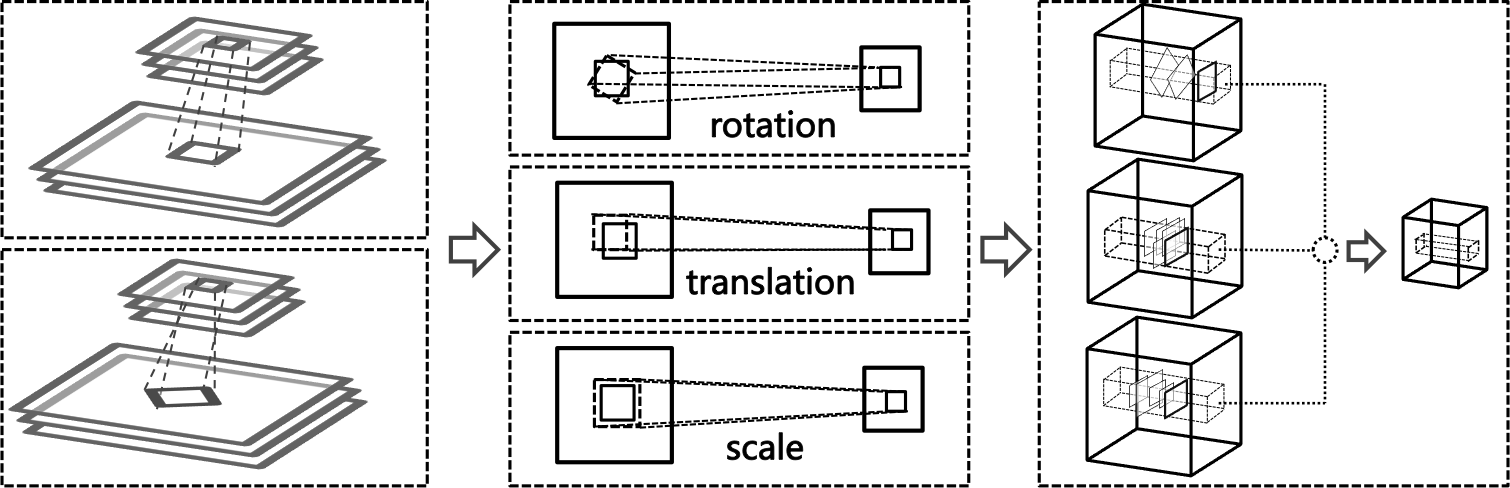
\includegraphics[width=1\linewidth]{sap_sap.png}
\caption{随机区域池化方法。}
\label{fig:sap_sap}
\end{figure}

随机区域池化主要由两个步骤组成:池化区域的选择和池化操作。首先,通过随机仿射变换对池化区域进行重采样。之后,在变换后的池化区域进行池化操作(均值池化、最大池化等),本章中采用的是最大池化。

不同于传统的池化方法,在一个固定的矩形区域进行池化操作,随机区域池化的池化区域通过仿射变换得到:$f : A {\rightarrow} B$,其中 $A {\in} \mathcal{R}^n$ 和 $B {\in} \mathcal{R}^m$ 代表两个仿射空间,假设 $x {\in} A$  代表一个 n 维向量。 仿射变换可以表示为 $f(x) = Tx + b$,其中 $T {\in} \mathcal{R}^{m \times n}$ 为仿射变换矩阵, $b {\in} B$ 为平移向量。对于二维图像空间的仿射变换,本章只考虑了最常见的平移、旋转、缩放三种变换以及它们之间的相互组合形式,用于随机区域池化的池化区域选择,如图~\ref{fig:sap_sap}所示。

假设 $\theta$ 代表旋转角,以向量 $[c_x, c_y]$ 为旋转中心, $[o_x, o_y]$ 为平移向量,$[s_x, s_y]$ 为缩放因子的仿射变换可以用一个七元组 $\{\theta, c_x, c_y, o_x, o_y, s_x, s_y\}$ 来表示,其变换公式可以形式化地表示为:
\begin{equation}  \label{equ:all}
  \left[
  \begin{array}{c}
          x' \\
          y' \\
          1
 \end{array}
 \right]
 =
  \left[
  \begin{array}{ccc}
          s_x \cos{\theta} & s_y \sin{\theta} & t_x\\
          -s_y \sin{\theta} & s_x \cos{\theta} & t_y\\
          0 & 0 & 1
  \end{array}
  \right]
  \left[
  \begin{array}{c}
          x \\
          y \\
          1
  \end{array}
  \right]
\end{equation}
\begin{equation} \label{equ:tx}
t_x = c_x (1 - s_x \cos{\theta}) - c_y s_y \sin{\theta} + o_x
\end{equation}
\begin{equation} \label{equ:ty}
t_y = c_x (1 + s_y \sin{\theta}) - c_y s_x \cos{\theta} + o_y
\end{equation}

随机区域的选择通过对上述七元组参数的随机采样获取,七元组参数服从如下概率分布:
\begin{equation} \label{equ:theta}
\theta \sim N(0, \sigma_{\theta}), 
\end{equation}
\begin{equation} \label{equ:cx}
c_x, c_y \sim N(0.5d, \sigma_{c})
\end{equation}
\begin{equation} \label{equ:sx}
s_x, s_y \sim N(1, \sigma_{s})
\end{equation}
其中 $d$ 代表输入特征图的高度或宽度;旋转角度、旋转中心、缩放因子分别服从以 0、$0.5d$、0为均值,
$\sigma_{\theta}$、$\sigma_c$ 、$\sigma_s$为标准差的高斯分布。三个标准差的大小直接影响了随机区域池化仿射变换的扰动幅度和特征増广的强度。

对池化区域进行仿射变换,变换后的池化区域往往被映射到非整数边界。双线性差值常用于对非整数边界上的特征进行估计。双线性插值,又称为双线性内插,在数学上,双线性插值是线性差值在二维空间的扩展,其核心思想是在两个方向分别进行一次线性插值。双线性插值会使特征的细节产生退化,但这种小幅度的退化反而有助于池化操作提取更具鲁棒性的特征。

对于前向传播的过程,根据式(\ref{equ:theta}), (\ref{equ:cx}), (\ref{equ:sx})随机生成一组七元组参数。这组参数唯一确定了一个仿射变换矩阵,对应于变换后的池化区域。随机区域池化采用双线性差值,在上述变换后的池化区域进行特征重采样。最后调用传统的最大池化或平均池化对重采样的特征进行池化操作,本章所采用的池化操作是最大池化,实际上平均池化同样适用于随机区域池化方法。前向传播过程的七元组参数是随机生成的,并不需要学习优化。

为了让网络可以端到端的学习,需要为前向传播过程设计相应的反向传播机制。前向传播根据生成的七元组参数,先进行特征空间的仿射变换,再通过双线性差值对特征进行重采样,最后调用最大池化生成池化结果。反向传播与之刚好相反,输出层误差经由最大池化、双线性差值即可传回输出层,实现整个网络端到端的学习。为了保证误差原路返回,每一轮反向传播需要与前向传播保持相同的空间仿射变换。

实际上,随机区域池化只是在传统的最大池化基础上,增加了一个随机池化区域仿射变换过程。对池化区域进行随机的仿射变化,在亚像素级别对特征进行重采样,生成一组具有随机平移、旋转和缩放的特征表达,以此来达到特征増广的效果,如图~\ref{fig:sap_sap}所示。当${\sigma_{\theta}=0}$,${\sigma_c=0}$, ${\sigma_s=0}$时,随机区域池化等价于最大池化。

随机区域池化仅用于网络的训练阶段,在测试阶段,为了保证测试结果的一致性,我们采用最大池化来代替随机区域池化。即强制令${\sigma_{\theta}=0}$,${\sigma_c=0}$, ${\sigma_s=0}$,跳过随机区域选择,直接进行最大池化。这样设计的目的是为了避免随机变量引起测试结果的不确定性,让大家可以更容易地复现出本章的实验结果。


\subsection{T形卷积网络结构}
\label{sec:sap:model:t}

\begin{figure} [t]
\centering
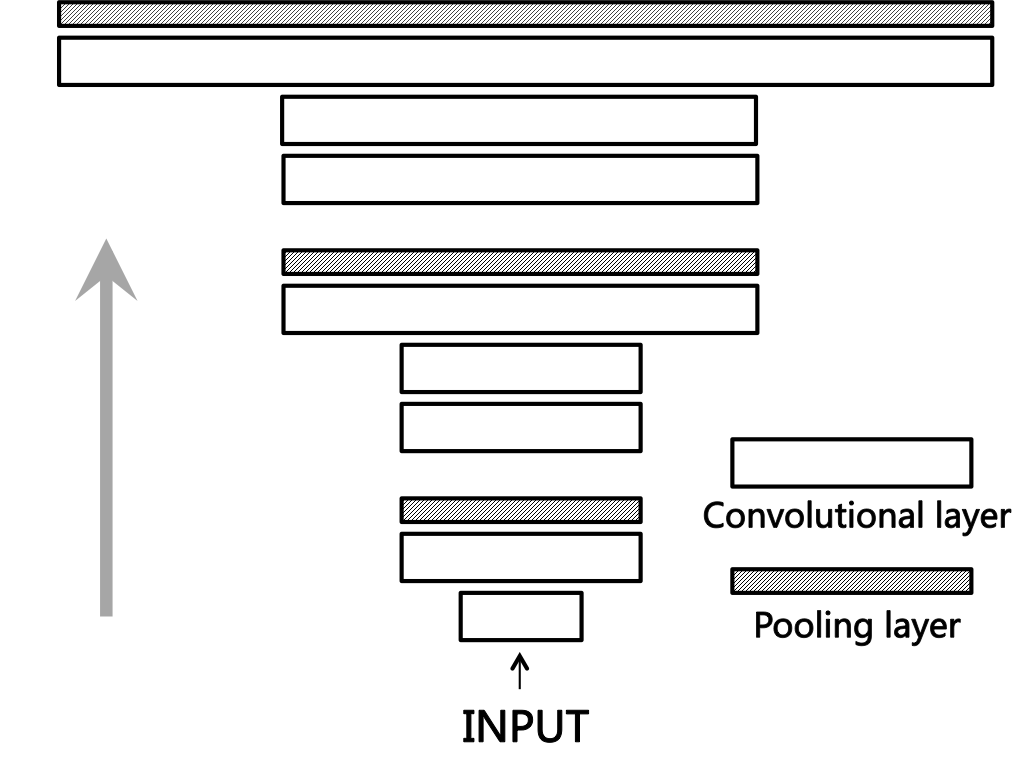
\includegraphics[width=0.7\linewidth]{sap_arc.png}
\caption{T型网络结构。}
\label{fig:sap_arc}
\end{figure}

除了池化策略之外,网络结构也会影响网络的特征表达能力。据我们了解,网络结构的设计还是经验主义的,并没有系统的理论依据。VGG~\cite{simonyan2014very} 和GoogLeNet~\cite{szegedy2014going,szegedy2015rethinking,szegedy2016inception}的成功启发我们,更深的网络结构、更小的感受野、合适的滑动步长均有助于网络性能的提升。最近He等人~\cite{he2015deep}的实验结果表明,随着网络深度的持续增加,网络的测试识别率会趋于饱和甚至下降。Szegedy等人~\cite{szegedy2015rethinking}建议,网络的设计应该避免特征表达瓶颈(Representational Bottleneck),特别在网络的初始阶段。实际上,如何确定网络的深度,保证网络的特征表达能力与计算复杂度;如何有效地组织卷积、池化、非线性化结构,来实现更优秀的泛化能力;如何设计每个卷积层感受野的大小和卷积核的个数,这些都是值得研究和探索的开放性问题。

\begin{table}[h]
{\caption{SAPNet 网络结构。表中一共定义四个SAPNet网络结构,SAPNet-$N$中的$N$代表与输入图像直接相连的第一个卷积层卷积核的个数。每一个SAPNet都是由三个T型结构、两个随机区域池化、一个全局均值池化、一个全连接层和一个Softmax层组成,八个卷积层被两个随机区域池化均匀隔开。}
\label{tab:model}}
\centering
\begin{tabular}{C{2.5cm}C{2.5cm}C{2.5cm}C{2.5cm}}
 \toprule[1.5pt]
\heiti{SAPNet-16} & \heiti{SAPNet-32} & \heiti{SAPNet-48} & \heiti{SAPNet-64} \\
\midrule[1pt]
conv3-16 & conv3-32 & conv3-48 & conv3-64 \\
conv3-32 & conv3-64 & conv3-96 & conv3-128 \\
\hline
\multicolumn{4}{c}{随机区域池化层} \\
\hline
conv3-32 & conv3-64 & conv3-96 & conv3-128 \\
conv3-32 & conv3-64 & conv3-96 & conv3-128 \\
conv3-64 & conv3-128 & conv3-192 & conv3-256 \\
\hline
\multicolumn{4}{c}{随机区域池化层} \\
\hline
conv3-64 & conv3-128 & conv3-192 & conv3-256 \\
conv3-64 & conv3-128 & conv3-192 & conv3-256 \\
conv3-128 & conv3-256 & conv3-384 & conv3-512 \\
\hline
\multicolumn{4}{c}{全局均值池化} \\
\hline
\multicolumn{4}{c}{全连接层} \\
\hline
\multicolumn{4}{c}{Softmax层} \\
 \bottomrule[1.5pt]
\end{tabular}
\end{table}

本节中,我们根据以往的实验经验,设计了一个通用的T形卷积网络结构,如图~\ref{fig:sap_arc} 所示。我们用长条状的立方体表示卷积层,立方体的长度代表卷积核的个数。不同于VGG网络在同一个阶段采用相同的特征维度进行分层的特征提取,T形结构与池化层相连的卷积层通道数会翻倍,此结构看起来像一个T形的倒金字塔,我们称之为T形网络结构。采用第~\ref{sec:sap:model:sap} 节随机区域池化和T型结构,我们设计了一组结构相似的SAPNet网络,如表~\ref{tab:model} 所示。表~\ref{tab:model} 中,一共定义四个SAPNet网络结构,SAPNet-$N$ 中的 $N$ 代表与输入图像直接相连的第一个卷积层卷积核的个数。每一个SAPNet都是由三个T型结构、两个随机区域池化、一个全局均值池化、一个全连接层和一个Softmax层组成,八个卷积层被两个随机区域池化均匀隔开。第一个T型结构中仅包换两个卷积层,这是因为相对于其他特征层,输入图片的尺寸最大,出于减少计算量的角度考虑,在第一个T型结构中只包含两层卷积。

在SAPNet中,所有的卷积都采用 $3\times3$ 大小的感受野,1 个像素的边界填充,1 个像素的滑动步长,这样的配置可以保证卷积操作不会改变特征图的空间维度。在随机区域池化层,我们采用 $2\times2$ 的池化区域大小和 2 个像素的滑动窗口步长,来实现4倍空间大小的特征下采样。最后采用全局均值池化来提取固定长度的特征。与其他图像识别任务一样,本章也采用Softmax对物体的类别进行预测。此外,对于所有的卷积层,我们依次采用批正则化BN~\cite{ioffe2015batch}对特征进行正则化处理,线性整流单元ReLU作为非线性激活函数,具有 0.1 丢弃率的Dropout来防止网络过拟合。值得注意的是,本章采用的BN操作与原论文~\cite{ioffe2015batch}的略有不同,我们省略了原文中BN的比例和平移操作,仅仅将BN作为对卷积特征的一种正则化。理论上,如果BN层紧邻卷积层之后,对卷积层的卷积核和偏执分别进行比例和平移变换,等价于BN层的比例和平移操作。

\begin{table*}
\centering
\caption{不同深度的卷积神经网络在CIFAR-10上的性能对比。}
\label{tab:layers}
\begin{tabular}{C{2.8cm}|C{0.9cm}C{0.9cm}C{0.9cm}C{0.9cm}C{0.9cm}C{0.9cm}C{0.9cm}C{0.9cm}C{1.cm}}%{c|ccccccccc}
 \hline
{\heiti 层数} & 6 & 7 & 8 & 9 & 10 & 11 & 12 & 13 & 14 \\
\hline
{\heiti 网络结构} & 2221 & 2321 & 2331 & 2431 & 2441 & 2541 & 2551 & 2651 & 2661\\
\hline
{\heiti 测试误差率 (\%)} & 10.09 & 8.77 & 8.53 & 8.35 & 7.93 & \bf{7.65} & 7.86 & 7.63 & 7.77\\
\hline
{\heiti 网络感受野} &  32 & 36 & 44 & 48 & 56 & 60 & 68 & 72 & 80\\
\hline
{\heiti 参数规模 (百万)} & 0.57 & 0.61 & 0.76 & 0.80 & 0.94 & 0.98 & 1.13 & 1.16 & 1.31 \\
\hline
\end{tabular}
\end{table*}

对于网络深度的选择,我们在CIFAR-10上进行了一组实验,实验结果如表~\ref{tab:layers} 所示,“网络结构”是对不同卷积网络结构的缩写。 例如 '2331' 指该网络结构为 8(2+3+3)个卷积层和 1 个全连接层,被 3 个最大池化分隔成 4 个部分,每个部分具有 2,3,3 个卷积层和 1 个全连接层,最后一个池化层是全局最大池化,提取具有固定长度的特征,最后通过Softmax来预测各类别的预测概率。如果不算全连接层,本章采用的SAPNet(如表~\ref{tab:model}所示) 网络深度为八。深度为八的网络并不是表~\ref{tab:layers} 中错误率最低的,但是综合考虑网络的识别率、计算量和参数数量,可以看出具有 8-11 层卷积的网络模型都是合适的选择,而八层网络具有最少的计算规模和参数数量,因此本章的所有实验都是基于八层卷积网络模型展开的。从表~\ref{tab:layers} 我们还可以看出,网络深度的选择与网络的感受野存在一定的关系。随着网络深度的增加,网络的感受野也逐渐增大,当网络的感受野增大到输入图片的 1.5-2.0 倍的时候,网络的识别能力达到峰值。继续增加网络的深度,对网络识别能力影响不大,额外增加的计算量与可学习参数并没有带来更高的回报与收益。在CIFAR-10,CIFAR-100,MNIST和SVHN这四个数据集上,输入图像的大小为 $32\times32$ 或 $28\times28$,一个 8-11 层深的卷积神经网络模型足以获取优越的识别与泛化能力。

为了解决特征瓶颈~\cite{szegedy2015rethinking}的问题,我们通过增加特征的通道数来缓解特征尺度上的锐减。特征的维度可以表示为特征的通道数与每张特征图的分辨率的乘积。一般情况下,从输入图像到最后一个卷积层,特征的维度应该缓慢的进行缩减。也就是说,我们应该避免特征维度大幅度的急剧压缩,以防止特征信息的快速流失。考虑到池化操作不会影响特征的通道数,但会成倍缩小特征图的分辨率,如果采用步长为 2 的滑动窗口进行池化,特征图分辨率会减小到原来的 $1/4$。由此可见,池化很有可能会导致特征因大幅度压缩而出现信息的过度流失,产生特征瓶颈问题。为了克服这个现象,我们提出了T型网络结构,通过增加与池化层直接相连的卷积层的通道数,来增加池化前特征的通道数,尽量降低池化过程中特征的信息流失。

SAPNet网络在设计的过程中,需要考虑的另一个问题是如何合理的分配网络的计算资源。卷积神经网络的大部分计算集中在卷积的乘法操作,而决定卷积层计算量的主要是输入特征的维度和卷积核参数。在池化前后,合理的分配输入输出特征图的通道数,可以有效地平衡网络在不同阶段的计算量。

\subsection{分析与讨论}
\label{sec:sap:model:discuss}

本章我们提出了一个用于图像识别任务的由随机区域池化和T形网络结构组成的SAPNet网络,该网络主要由两个随机区域池化与三个T型网络结构搭建而成。

受数据増广的启发,为了提高网络的泛化能力,我们将数据増广思想推广到特征层,提出了随机区域池化方法。通过随机仿射变换对池化区域进行扰动,生成一组具有随机平移、旋转和缩放的特征表达,扩大了特征的表示范围,增加了特征的多样性。随机区域池化方法并不需要对仿射变换参数进行优化求解,整个计算过程十分简单快速,并未引入过多的额外计算开销,是一种计算代价很小的提升网络泛化能力的方法。值得注意的是,随机区域池化并不是一种增强特征不变性的方法,而是通过特征増广来增强网络泛化能力,防止网络过早出现过拟合现象。本章中采用最大池化对随机区域内的特征进行池化,相当于在最大池化的基础上,对输出特征进行了合理的扰动。同样地,均值池化等其他池化方法也可以与随机区域池化配合使用,达到特征増广的效果。

此外,本章提出了T型网络结构,并以此为基础设计出SAPNet网络。不同于其他网络模型仅仅在全连接层使用Dropout,SAPNet在每个卷积层都采用一个丢失率较小的Dropout对特征进行正则化,防止网络过早地进入过拟合状态。实验结果表明,这样的配置同样可以保证网络的泛化能力。


\section{实验结果}
\label{sec:sap:experiment}

基于深度学习框架caffe~\cite{jia2014caffe},我们实现了本章提出的随机区域池化和T型网络模型。所有的实验都以数据并行的方式运行于具有两颗GPU核心的单卡K80服务器上。我们在四个图像识别数据集CIFAR-10,CIFAR-100,MNIST,和SVHN上对多组不同参数大小的SAPNet进行了测试,在CIFAR-10数据集上,我们设计了更多的对比实验来验证随机区域池化和T型网络结构的有效性。

在所有实验中,我们采用批大小(Batch Size)为 96 的随机梯度下降算法来训练网络。网络的初始学习率为 0.01,训练过程中学习率会逐渐减小,每次缩小为原来的 $1/10$,持续缩小 3 次,直到学习率降低到 1e-5。训练过程中,采用 0.9 的动量因子(Momentum)和 0.004 的权重衰减因子(Weight Decay )进行参数更新。对于随机区域池化层,七元组的各参数标准差设为$\sigma_{\theta}=5^{\circ}$,$\sigma_c=0.25d$,$\sigma_s=0.01$。采用与第~\ref{sec:sap:experiment:param}节相同的数据预处理方式,即对每张图像,减去训练集图像的BGR均值,作为整个网络的输入,且并不对图像进行归一化或白化处理。

\subsection{CIFAR-10}
\label{sec:sap:cifar10}

我们首先在CIFAR-10~\cite{krizhevsky2009learning}数据集上,对随机区域池化与T型网络的有效性进行验证。CIFAR-10 由 60,000 张 $32\times32$ 大小的 10 类彩色图像构成,整个数据集被平均分成 6 份,每份 10,000 张图片,其中 5 份作为训练数据,1 份作为测试数据。

\begin{table}[h]
\centering
\caption{随机区域池化与其他池化方法的对比试验。}
\label{tab:others}
%\begin{tabular}{C{3cm}C{2cm}C{2cm}}
 \begin{tabular}{lcc}
 \toprule[1.5pt]
{\heiti 模型} & {\heiti 参数规模} & {\heiti 测试错误率(\%)} \\
\midrule[1pt]
SAPNet-32(最大池化) & 0.76 M & 8.53 \\
SAPNet-32(均值池化) & 0.76 M & 8.13 \\
SAPNet-32(随机池化) & 0.76 M & 8.50 \\
\hline
SAPNet-32(随机区域池化) & 0.76 M & \bf{7.56} \\
 \bottomrule[1.5pt]
\end{tabular}
\end{table}

\begin{table}[b]
\centering
\caption{不同参数规模下随机区域池化与最大池化性能对比。}
\label{tab:max}
%\begin{tabular}{C{3cm}C{2cm}C{2cm}}
\begin{tabular}{lcc}
 \toprule[1.5pt]
{\heiti 模型} & {\heiti 参数规模} & {\heiti 测试错误率(\%)} \\
\midrule[1pt]
SAPNet-32(最大池化) & 0.76 M & {8.53} \\
SAPNet-48(最大池化) & 1.71 M &{7.69} \\
SAPNet-64(最大池化) & 3.03 M & {7.01} \\
\hline
SAPNet-32(随机区域池化) & 0.76 M & {7.56} \\
SAPNet-48(随机区域池化) & 1.71 M &{7.02} \\
SAPNet-64(随机区域池化) & 3.03 M & {6.61} \\
 \bottomrule[1.5pt]
\end{tabular}
\end{table}

随机区域池化与其他池化方法的对比结果如表~\ref{tab:others} 所示。实验中,我们采用了与 SAPNet-32(表~\ref{tab:model})相同的八层卷积网络结构,分别用最大池化、均值池化、随机池化来代替 SAPNet-32 中的随机区域池化。在没有数据増广的情况下,表~\ref{tab:others} 中所有的实验都达到了一个极高的识别率。由此可见,T形网络结构本身就具备强大的特征表达能力。在相同的网络结构、参数规模和计算量的基础上,随机区域池化方法明显优于最大池化、均值池化和随机池化。从本组对比实验结果可以看出,在网络的泛化能力上,随机区域池化 > 均值池化 > 随机池化 > 最大池化。由此可见,相对于最大池化、均值池化和随机池化,随机区域池化可以有效地增强网络的泛化能力,提升网络的识别结果。


\begin{table}[!h]
\centering
\caption{CIFAR-10数据集上与已有模型的对比实验。}
\label{tab:cifar10}
%\begin{tabular}{C{4.5cm}C{1cm}C{2cm}}
\begin{tabular}{L{6cm}cc}
 \toprule[1.5pt]
{\heiti 模型} & {\heiti 参数规模} & {\heiti 测试错误率(\%)} \\
\midrule[1pt]
\multicolumn{3}{c}{\heiti 没有数据増广} \\
\hline
Maxout~\cite{goodfellow2013maxout} & $>$5 M & 11.68 \\
Prob maxout~\cite{springenberg2013improving} & $>$5 M & 11.35 \\
DasNet~\cite{stollenga2014deep} &  $>$5 M & 9.22 \\
NIN~\cite{DBLP:journals/corr/LinCY13} & 0.97 M & 10.41 \\
DSN~\cite{lee2015deeply} & 0.97 M &9.69 \\
%RCNN-96~\cite{liang2015recurrent} & 0.67 M & 9.31 \\
%RCNN-128~\cite{liang2015recurrent} & 1.19 M & 8.98 \\
RCNN~\cite{liang2015recurrent} & 1.86 M & 8.69 \\
ALL-CNN~\cite{springenberg2015striving} & 1.3 M & 9.08 \\
Tree+Max-Avg~\cite{lee2015generalizing} & 1.85M & 7.62 \\
DenseNet~\cite{huang2016densely} & 15.3M & \bf{5.19} \\
\hline
SAPNet-32 & 0.76 M & \bf{7.56} \\
SAPNet-48 & 1.71 M &\bf{7.02} \\
SAPNet-64 & 3.03 M & \bf{6.36(6.50$\pm$0.14)} \\
\midrule[1pt]
\multicolumn{3}{c}{\heiti 有数据増广} \\
\hline
Maxout~\cite{goodfellow2013maxout} & $>$5 M & 9.38 \\
Prob maxout~\cite{springenberg2013improving} & $>$5 M & 9.39 \\
dasNet~\cite{stollenga2014deep} &  $>$5 M & 9.22 \\
DropConnect~\cite{wan2013regularization} & 5 networks & 9.32 \\
NIN~\cite{DBLP:journals/corr/LinCY13} & 0.97 M & 8.81 \\
DSN~\cite{lee2015deeply} & 0.97 M & 7.97 \\
%RCNN-96~\cite{liang2015recurrent} & 0.67 M & 7.37 \\
%RCNN-128~\cite{liang2015recurrent} & 1.19 M & 7.24 \\
RCNN~\cite{liang2015recurrent} & 1.86 M & 7.09 \\
Highway network~\cite{srivastava2015training} & 2.3 M & 7.54(7.72$\pm$0.16) \\
ALL-CNN~\cite{springenberg2013improving} & 1.3 M & 7.25 \\
%ResNet-20~\cite{he2015deep} & 0.27 M & 8.75 \\
%ResNet-32~\cite{he2015deep} & 0.46 M & 7.51 \\
%ResNet-44~\cite{he2015deep} & 0.66 M & 7.17 \\
%ResNet-56~\cite{he2015deep} & 0.85 M & 6.97 \\
ResNet~\cite{he2015deep} & 1.7M & {6.43(6.61$\pm$0.16)} \\
Fitnet4-LSUV~\cite{mishkin2015all} & 2.5M & 6.06 \\
Tree+Max-Avg~\cite{lee2015generalizing} & 1.85M & 6.05 \\
Tuned CNN~\cite{snoek2015scalable} & 1.29M & 6.37 \\
DenseNet~\cite{huang2016densely} & 25.6M & \bf{3.46} \\
\hline
SAPNet-32 & 0.76 M & {6.77} \\
SAPNet-48 & 1.71 M & \bf{5.92} \\
SAPNet-64 & 3.03 M & \bf{5.57(5.66$\pm$0.09)} \\
\midrule[1pt]
\multicolumn{3}{c}{\heiti 超大规模数据増广} \\
\hline
Large ALL-CNN~\cite{springenberg2014striving} & - & 4.41 \\
Fractional MP~\cite{graham2014fractional} & - & \bf{3.47} \\
 \bottomrule[1.5pt]
\end{tabular}
\end{table}

为了更直观地理解随机区域池化对网络泛化能力的提升幅度,我们进行了多组随机区域池化与最大池化的对比实验,实验结果如表~\ref{tab:max} 所示。在具有相同网络结构、参数规模和计算复杂度的情况下,随机区域池化均优于最大池化。并且一个有趣的发现是,SAPNet-32(随机区域池化)的性能要好于比它的参数规模与计算量大一倍的SAPNet-48(最大池化);SAPNet-48(随机区域池化)的性能与比它的规模大近一倍的SAPNet-64(最大池化)基本持平。由此可见,采用随机区域池化带来的网络性能提升,近似于网络增加了接近一倍的额外参数与计算量所能达到的效果。


最后,我们对比了SAPNet与其他曾经在CIFAR-10上取得过优异成绩的网络模型,实验结果如表~\ref{tab:cifar10}所示。我们对三组具有不同参数规模的SAPNet进行了测试,在没有数据増广的情况下,三组模型均取得了较高的物体识别精度。具有相近参数规模的两个网络,SAPNet-48取得了7.02\%的测试错误率,优于Tree+Max-Avg~\cite{lee2015generalizing}。SAPNet-64取得了 6.36\% 的测试错误率,仅次于DenseNet~\cite{huang2016densely}。为了避免单次实验的偶然性,我们对SAPNet-64重复进行了五次重复实验,以保证实验结果的可靠性。


特征増广与数据増广是两个不同的概念,对于采用了随机区域池化的网络模型,数据増广依然有效,并且可以进一步提高网络的泛化能力。为此,我们增加了多组在具有数据増广情况下CIFAR-10数据集的实验结果,如表~\ref{tab:cifar10} 所示。与之前的工作~\cite{goodfellow2013maxout,springenberg2013improving,stollenga2014deep,wan2013regularization,DBLP:journals/corr/LinCY13,lee2014deeply,liang2015recurrent,srivastava2015training,springenberg2014striving}相同,我们通过随机平移和水平翻转对CIFAR-10数据集的训练图像进行数据増广。测试时,从测试图像的四角和中心分别截取 $24\times24$ 像素大小的五张图片,并对其进行水平翻转,即对一共十张图片进行测试,最终的测试结果是十张图片预测概率的均值。实验结果如表~\ref{tab:cifar10} 所示,在具有数据増广的情况下,SAPNet-32 取得了 6.77\% 的测试误差,比没有数据增广的 SAPNet-32 提高了 0.79\%;同样的 SAPNet-48 相比于没有数据增广提升了 1.1\%;SAPNet-64以 5.57\% 的测试错误率,排在第二名。由此可见,数据增广对随机区域池化仍然适用,特征增广和数据增广虽然采用了类似的思想,但具有不同的效果。

\begin{table}[t]
\begin{center}
\caption{CIFAR-100数据集上与已有模型的对比实验。}
\label{tab:cifar100}
\begin{tabular}{L{6cm}cc}
 \toprule[1.5pt]
{\heiti 模型} & {\heiti 参数规模} & {\heiti 测试错误率(\%)} \\
\midrule[1pt]
\multicolumn{3}{c}{\heiti 没有数据増广} \\
\hline
Maxout~\cite{goodfellow2013maxout} & $>$5 M & 38.57 \\
Prob maxout~\cite{springenberg2013improving}  & $>$5 M & 38.14 \\
DasNet~\cite{stollenga2014deep} & $>$5 M & 33.78 \\
Tree based priors~\cite{srivastava2013discriminative} & - & 36.85 \\
NIN~\cite{DBLP:journals/corr/LinCY13} & 0.98 M & 35.68 \\
DSN~\cite{lee2015deeply}  & 0.98 M & 34.57 \\
%RCNN-96~\cite{liang2015recurrent} & 0.67 M & 34.18 \\
%RCNN-128~\cite{liang2015recurrent} & 1.19 M & 32.59 \\
RCNN~\cite{liang2015recurrent}  & 1.87 M & {31.75 }\\
ALL-CNN~\cite{springenberg2013improving} & 1.30 M & 33.71 \\
Tree+Max-Avg~\cite{lee2015generalizing} & 1.76 M & 32.37 \\
ELU-Network~\cite{clevert2015fast} & 39.32 M & 24.28 \\
DenseNet~\cite{huang2016densely} & 15.3M & \bf{19.64} \\
\hline
SAPNet-32 & 0.76 M & {32.22} \\
SAPNet-48 & 1.71 M &{29.32} \\
SAPNet-64 & 3.03 M & \bf{27.59} \\
\midrule[1pt]
\multicolumn{3}{c}{\heiti 具有数据増广} \\
\hline
Highway Network~\cite{srivastava2015training} & 2.30 M & 32.24 \\
Fitnet4-LSUV~\cite{mishkin2015all} & 2.5 M & 27.66 \\
Tuned CNN~\cite{snoek2015scalable} & 1.29 M & 27.40 \\
DenseNet~\cite{huang2016densely} & 25.6M & \bf{17.18} \\
\hline
\multicolumn{3}{c}{{\bf{Extreme}} data augmentation} \\
\hline
Fractional MP~\cite{graham2014fractional} & - & 26.39 \\
 \bottomrule[1.5pt]
\end{tabular}
\end{center}
\end{table}

值得一提的是,CIFAR-10数据集上取得的最好结果是Graham等人~\cite{graham2014fractional}提出的Fractional MP。但是Graham等人对CIFAR-10进行了超大规模的数据増广,包括对输入图像的平移、旋转、水平翻转、拉伸、错切等。

\subsection{CIFAR-100}
\label{sec:sap:cifar100}

CIFAR-100~\cite{krizhevsky2009learning}是一个类似于CIFAR-10的具有 100 类物体的图像数据集。使用相同的网络结构和配置参数,在没有特征増广的情况下,我们在CIFAR-100上对SAPNet-32、SAPNet-48和SAPNet-64进行了测试,实验结果如表~\ref{tab:cifar100}所示。SAPNet-64取得了 27.59\% 的测试错误率,仅次于ELU-Network~\cite{clevert2015fast},但是我们仅使用了相对于ELU-Network网络模型8\%的参数数量。在没有数据増广的情况下,27.59\% 的测试错误率已经是CIFAR-100数据集上第二好的实验结果。

CFFAR-100数据集上,每个类别只具有500个训练样本。这样的样本数量对于大规模的卷积神经网络来说是远远不够的,较小的样本数量使得网络参数的训练不够充分,尤其是对于深层的网络参数。在参数反向传播参数更新的过程中,深层网络参数的回传梯度相对较大,使得深层网络参数更新幅度较大。而对于浅层网络,由于梯度弥散的原因,回传的梯度值较小,参数的更新较为缓慢。对于网络浅层的参数,学习到的往往是图像的边缘和角点等低级特征。对于这些网络浅层的卷积核参数,因为学习的是相对通用的图像低级特征,所有输入图像均能为浅层的参数更新有所贡献。但是对于网络的深层的参数,学习到的往往是图像的纹理特征、局部特征、甚至类别相关的全局特征。对于这些类别相关的网络参数的学习与更新,需要大量的同类别训练样本。因此,对于像CFFAR-100数据集这样,单类别训练样本很少的数据集,卷积神经网络的识别效果往往不尽人意。


\subsection{MNIST}
\label{sec:sap:mnist}

\begin{table}[h]
\begin{center}
\caption{MNIST数据集上与已有模型的对比实验。}
\label{tab:mnist}
%\begin{tabular}{C{4.5cm}C{1cm}C{2cm}}
\begin{tabular}{L{6cm}cc}
 \toprule[1.5pt]
{\heiti 模型} & {\heiti 参数规模} & {\heiti 测试错误率(\%)} \\
\midrule[1pt]
\multicolumn{3}{c}{\heiti 没有数据増广} \\
\hline
Maxout~\cite{goodfellow2013maxout} & 0.42 M & 0.45 \\
NIN~\cite{DBLP:journals/corr/LinCY13} & 0.35 M & 0.47 \\
DSN~\cite{lee2015deeply} & 0.35 M & 0.39 \\
RCNN~\cite{liang2015recurrent} & 0.67 M & \bf{0.31} \\
Tree+Max-Avg~\cite{lee2015generalizing} & 1.85 M & \bf{0.31} \\
FitNet-LSUV-SVM~\cite{mishkin2015all} & 0.03 M & 0.38 \\
\hline
SAPNet-16 & 0.19 M & {0.31} \\
SAPNet-32 & 0.76 M &\bf{0.29} \\
\midrule[1pt]
\multicolumn{3}{c}{\heiti 具有数据増广} \\
\hline
DropConnect~\cite{wan2013regularization} & 5 networks & 0.21 \\
MCDNN \cite{ciresan2012multi} & 35 networks & 0.23 \\
 \bottomrule[1.5pt]
\end{tabular}
\end{center}
\end{table}

MNIST~\cite{lecun1998gradient}手写体数据集相对比较简单,因此,我们从表~\ref{tab:model} 中选择了两个规模最小的网络SAPNet-16和SAPNet-32进行了测试,实验结果如表~\ref{tab:mnist} 所示。采用与CIFAR-10相同的设置参数,具有大约 0.19M 参数的SAPNet-16取得了 0.31\% 的测试错误率,该结果与具有 0.67M 参数的RCNN-96~\cite{liang2015recurrent}持平。此外,更大规模的网络模型SAPNet-32取得了 0.29\% 的测试误差。在不考虑数据増广的情况下,该结果优于其他网络模型。

MNIST数据集上的最好测试结果是0.21\%,该记录是2013年Wan等~\cite{wan2013regularization}人提出的DropConnect取得的,Wan等人采用复杂的数据増广和多模型(五个网络)平均的方法,一直保持着MNIST数据集的最佳记录。

\subsection{SVHN}
\label{sec:sap:svhn}

SVHN~\cite{netzer2011reading} 的图片采集自真实环境,也是一个数字识别数据集,但是由于图像的亮度变化比较剧烈,分类和识别难度要比MNIST大很多。采用与Goodfellow~\cite{goodfellow2013maxout}类似的训练步骤,我们在SVHN数据集上,对SAPNet-32、SAPNet-48和SAPNet-64 三个具有不同参数规模的网路进行了测试,实验结果如表~\ref{tab:svhn} 所示。从实验结果可以看出SAPNet-64取得了1.71\%的测试误差率,比Tree+Max-Avg~\cite{lee2015generalizing} 低了0.02\%,比DenseNet~\cite{huang2016densely}低了0.12\%。

\begin{table}
\begin{center}
\caption{SVHN数据集上与已有模型的对比实验。}
\label{tab:svhn}
%\begin{tabular}{C{4.5cm}C{1cm}C{2cm}}
\begin{tabular}{L{6cm}cc}
 \toprule[1.5pt]
{\heiti 模型} & {\heiti 参数规模} & {\heiti 测试错误率(\%)} \\
\midrule[1pt]
\multicolumn{3}{c}{\heiti 没有数据増广} \\
\hline
Maxout~\cite{goodfellow2013maxout}  & $>$5 M & 2.47 \\
Prob maxout~\cite{springenberg2013improving} & $>$5 M & 2.39 \\
NIN~\cite{DBLP:journals/corr/LinCY13} & 1.98 M & 2.35 \\
DSN~\cite{lee2015deeply} & 1.98 M & 1.92 \\
%RCNN-128 & 1.19 M & 1.87 \\
%RCNN-160 & 1.86 M & 1.80 \\
RCNN~\cite{liang2015recurrent} & 2.67 M & {1.77} \\
Tree+Max-Avg~\cite{lee2015generalizing} & 4.00M & 1.69 \\
DenseNet~\cite{huang2016densely} & 27.2M & \bf{1.59} \\
\hline
SAPNet-32 & 0.76 M & {1.87} \\
SAPNet-48 & 1.71 M & {1.75} \\
SAPNet-64 & 3.03 M & \bf{1.71} \\
\hline
\multicolumn{3}{c}{\heiti 具有数据増广} \\
\hline
Multi-digit number recognition~\cite{goodfellow2013multi} & $>$5 M & 2.16 \\
DropConnect~\cite{wan2013regularization} & 5 networks & 1.94 \\
 \bottomrule[1.5pt]
\end{tabular}
\end{center}
\end{table}

\section{本章小结}
\label{sec:sap:conclude}


本章提出了具有T形网络结构和随机区域池化的卷积网络结构SAPNet。通过对传统池化区域进行随机仿射变换,在不影响特征空间特征分布的情况下对池化特征进行扰动,扩展特征空间,增加特征的多样性,最终达到特征増广的目的。此外,我们还提出了T型网络结构,通过增加池化层之前的特征维度,可以有效地避免特征表达瓶颈问题。最后,我们在CIFAR-10,CIFAR-100,MNIST和SVHN四个数据集上对SAPNet进行了测试,实验结果表明随机区域池化的识别能力优于均值池化、最大池化和随机池化,具有较好的泛化能力。在没有数据増广的情况下,SAPNet在MNIST上取得了最好的识别性能,在CIFAR-10、CIFAR-100和SVHN排名第二。且数据增广对SAPNet仍然适用,虽然特征增广与数据增广基于相似的思想甚至实现手段,但是两种方法互不排斥,均能提高整个网络的泛化能力。














